
\section{Cluster}

Die Evaluation wurde auf dem Rechencluster des Lehrstuhl für Betriebssysteme der Heinrich-Heine Universität Düsseldorf durchgeführt.
Das Cluster besitzt mehrere Knoten die Nutzer reservieren und benutzen können.

Die zur Evalutation verwendeten Knoten haben den Xeon E3-1220 Prozessor, bezitzen 16Gigabyte Arbeitsspeicher und eine 240 Gigabyte SSD.
Alle Knoten im Cluster sind mit Gigabit-Ethernet verbunden und können miteinander kommunizieren. 

Das home-Verzeichnis eines Nutzer ist in einem verteilten Dateisystem gespeichert. Damit können Dateien im home-Verzeichnis, unabhänging davon welcher Knoten genutzt wird, gelesen werden.

\section{Testdaten}


Als Testdatensatz wird ein Teil des Microsoft Acadmic Graph genutzt \cite{sinha2015an}. Der Graph enthält wissenschaftliche Publikationen und die Zitierungsbeziehungen zwischen diesen Publikation, sowie Autoren, Institutionen, Journals, Konferenzen und Forschungsgebieten.

In dem Testdatensatz werden nur die Zitierungen zwischen Journals betrachtet. Dabei sind nur Journals enhalten, in denen zwischen 2007 und 2011 mehr als 100 Paper veröffentlicht wurden und die mindestens auf andere Journals fünf mal verwiesen haben.
Der Datensatzt besteht aus einer Kantendatei, in die die Verweise von einem Journal auf ein anderes darstellen. Dabei speichert jede Kante welches Journals auf welches verweist, in welchem Forschungsgebiet, in welchem Jahr und die Anzahl der Verweise.

Die verschiedene Forschungsgebiete stellen dabei die Layer des Graphen dar.

Die Kantendatei besteht aus 34715307 Kanten, die zwischen 12670 Journals in 12611 Layern liegen.


\section{Benchmarks}

Um die Perfomance des MultiLayer Systems in GE zu testen, wurden für verschiedenen Funktionen Benchmarks durchgeführt. Um zu prüfen, wie sich die Perfomance mit unterschiedlicher Anzahl von Servern verändert,
wurde jeder der Benchmarks mit 1 bis 8 Servern durchgeführt. Bei allen Benchmarks ist die Proxy für das Messen der Laufzeit verantwortlich.

Es wird das Laden der Kantendatei, das Berechnen der Graph Dichte und das Berechnen der Hub und Authority Werte untersucht. Die Funktionen für die Benchmarks wurden ausgewählt, um die Performance für verschiedene Arten der Berechungen zu testen.

Bei der Berechnung der Dichte handelt es sich um eine Funktion, bei der die Server nicht untereinander kommunizieren müssen. Jeder Server berechnet sein lokales Ergebnis für die Knoten, die er speichert und sendet dieses an die Proxy. 
Diese aggregiert am Ende das Geamtergbeniss. Hier lässt sich prüfen, wie sich die Laufzeit verhält, wenn die Server für die Ausführung nicht miteinander kommunizieren müssen.

Bei der Berechnung der Hub und Authority Werte müssen die Server viel untereinander kommunizieren. Sie führen soweit es geht die Aktualisierungen der Werte lokal durch, müssen aber, falls sie entfernte Knoten aktualisieren müssen oder die Werte von entfernten Knoten benötigt werden, diese von den anderen Servern erhalten.
Die Proxy koordiniert hierbei nur die Ausführung der einzelnen Aktualisierungen und Normalisierung der Wert. Hiermit wird geprüft, wie sich die Laufzeit verhält, wenn einiges an inter Server Kommunikation nötig ist.


\subsection{Ladezeiten}

Um die Ladezeit zu messen, wurde der Ladevorgang jeweils mit 1-8 Servern durchgeführt. Dabei wurde für jede Konfiguration 5 Durchläufe gemacht und der Mittelwert gebildet.

Die Ladezeit verbessert sich mit einer steigenden Anzahl an Servern von knapp 8 Minuten auf nur 1,5 Minuten. Dabei ist zu beobachten, dass die bei 5 Servern stagniert und sich nur minimal verändert.

Dies ist wie folgt zu begründen: Beim Laden liest jeder Server die Kantendatei komplett, während er parallel die Knoten für die er verantwortlich ist in GE speichert. Hat man nur einen Server, ist dieser für alle Knoten verantwortlich
und das Speichern der Knoten dauert deutlich länger, als das Lesen der Kantendatei. Bei einer höheren Serveranzahl bleibt die Zeit zum Lesen der Kantendatei gleich, während die Anzahl der Knoten die jeder Server speichern muss sinkt.
Ab dem Punkt, wo das Lesen der Kantendatei länger dauert, als das Speichern der Knoten, lässt sich keine Verbesserung durch mehr Server erreichen. Für eine noch größere Kantendatei wäre zu erwarten, dass es mehr Server benötigt, um den Punkt zu erreichen, wo die Verbesserung stagniert.

\begin{figure}
  \centering
  \begin{subfigure}[b]{1.0\textwidth}
    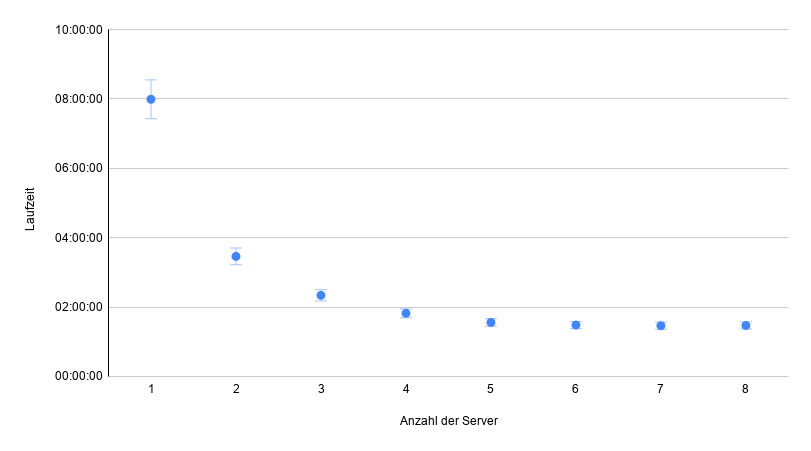
\includegraphics[width=1.0\linewidth]{img/eval_load.png}
  \end{subfigure}
  \caption{Einzelne Grafik (centered)}
  \label{eval:load}
\end{figure}

\subsubsection{Graph Dichte}

Bei der Graphdichte wurden für jede Konfiguration an Servern jeweils 10 Durchläufe gemessen und der Mittelwert gebildet. Die Ergebnisse sind in Abbildung \ref{eval:density} gezeigt.

Die Zeit, um die Graphdichte zu berechnent, sinkt von 11.47 Sekunden auf 2.19 Sekunden. Umso größer die Anzahl der Server desto geringer ist die Anzahl an Knoten, für die ein einzelner Server verantwortlich ist. Damit sinkt auch der Aufwand für jeden einzelnen Server, umso mehr Server beteiligte sind. 
Diese Entwicklung lässt sich in den Werten gut beobachten. Besonders der Sprung von einem zu zwei Servern halbiert knapp die Laufzeit zur Berechnung der Graphdichte.

\begin{figure}
  \centering
  \begin{subfigure}[b]{1.0\textwidth}
    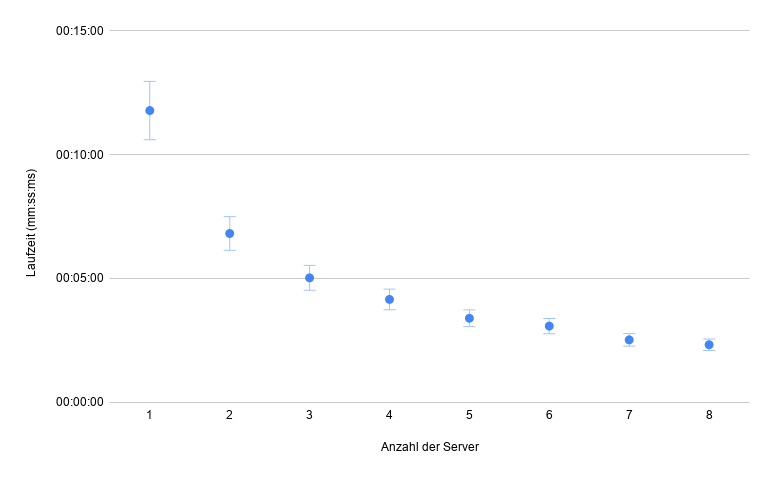
\includegraphics[width=1.0\linewidth]{img/eval_density.png}
  \end{subfigure}
  \caption{Einzelne Grafik (centered)}
  \label{eval:density}
\end{figure}



\subsubsection{HITS}

Bei HITS wurde für jede Konfiguration jeweils die Dauer von 5 Update Runden für Hub und Authority Werte gemessen und der Mittelwert dieser gebildet. Die Ergebnisse sind in Abbildung \ref{eval:hits} gezeigt.

Die Zeit für eine Update Runde wird mit steigender Serveranzahl immer geringer. Auch hier sinkt für jeden Server mit der Anzahl an Knoten, für die er verantwortlich ist die Arbeit, die er bewältigen muss.

Jedoch sorgen mehr Server auch dafür, dass mehr Netzwerknachrichten zwischen ihnen ausgetauscht werden müssen.
Die Server müssen bei jeder Update Runde miteinander kommunizieren, um entweder die Werte von entfernten Knoten anzufragen oder diese an andere Server zu senden. 
Diese Kommunikation ist allerdings optimiert, indem die Anfragen für die Werte von entfernten Knoten immer nur gebündelt verschickt werden und so das Senden vieler kleiner Nachrichten vermieden wird.



\begin{figure}
  \centering
  \begin{subfigure}[b]{1.0\textwidth}
    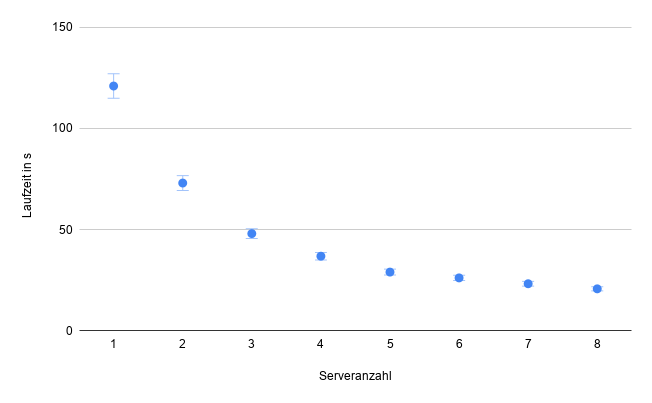
\includegraphics[width=1.0\linewidth]{img/eval_hits.png}
  \end{subfigure}
  \caption{Einzelne Grafik (centered)}
  \label{eval:hits}
\end{figure}
